%!TEX root = index.tex

\chapter{Flights Scheduling}

\red{TODO}
% že to je zjednodušení problému na 1 rwy
% co je vlastně kritérium
% různé pořadí různých tříd má různé trvání
% popis obrázků plánů
% posun jen doprava ne dřív
% není to project schedulling protože tady to není jednosměrně, když jsou sloty opačně, tak platí jiná podmínka
% nemůžu použít nic z KOčka - popsat co a proč
% nemůžu použít online algoritmy
% většina z nich počítá s tím, že arrival time a release time jsou stejné, u mně jsou různé,
% Shortest processing time first nemůžu použít, protože processing times nejsou konstantní
% není preempce 
%nejde nám o optimální řešení ale good enough které se podobá reálnému řídícímu

\section{Slot Selection}

\subsection{Algorithm 1}

\begin{figure}[h]
    \centering
    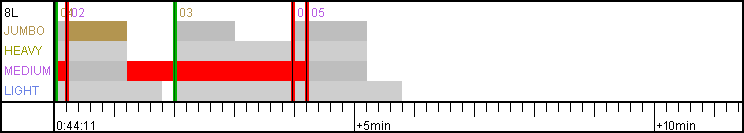
\includegraphics[width=\textwidth]{figures/rwy-in-place.png}
    \caption{Example of runway plan with colliding slots}
    \label{fig:rwy-in-place}
\end{figure}

An example of a plan generated by Algorithm 1 is shown in Figure \ref{fig:rwy-in-place}. This algorithm is the simplest of all implemented, it doesn't perform any deliberation on where to put the slot in the plan and simply places it in the time the aircraft is expected to arrive, ignoring possible collisions with other aircraft. This algorithm is obviously no good for actual use and serves only for comparison to other algorithms and to allow analysing of the traffic flow: it shows how many collisions there are or if the planes arrive to the runway periodically or in groups.

\subsection{Algorithm 2}

\begin{figure}[h]
    \centering
    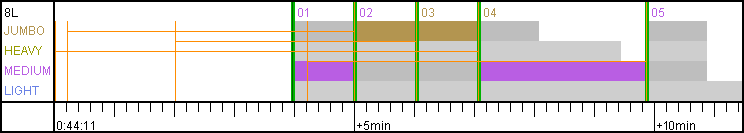
\includegraphics[width=\textwidth]{figures/rwy-end.png}
    \caption{Example of runway with slots in the order of plane's first appearance}
    \label{fig:rwy-end}
\end{figure}

Second algorithm is the simplest one that guarantees no collisions will take place between aircraft. When new plane appears on radar screen it's slot is created after all previously planned slots and not sooner than at the plane's minimal estimated time of arrival.

Figure \ref{fig:rwy-end} shows an example of a plan generated by this algorithm. It is clearly visible that unnecessary delays can occur when the interval between when the plane shows on the radar and its ETA differ from plane to plane. This can happen when the arrival routes have different lengths. Approach route for airplane heading directly to runway will be much shorter than for airplane arriving from opposite direction, because such plane must first fly around the airport before landing. \red{ref to figure with KATL approach routes} In the example shown on Figure \ref{fig:rwy-end} flight \texttt{TRS753} will arrive more than 5 minutes late because it appeared on the radar screen later than flights \texttt{TRS1341} and \texttt{DAL1946}.

\subsection{Algorithm 3}

\begin{figure}[h]
    \centering
    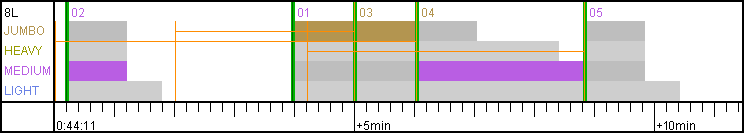
\includegraphics[width=\textwidth]{figures/rwy-fill-voids.png}
    \caption{Example of runway plan with slots fixed in place}
    \label{fig:rwy-fill-voids}
\end{figure}

Algorithm 3 creates the slot for arriving airplane in the first empty space following planes estimated arrival time the slot fits in. The wake turbulence separation minima is taken into account for both preceding and following slot so no collisions between slots occur. The advantage of this this algorithm is its simplicity and the fact that the planed slots are fixed. This means that if the controller assigns a slot to airplane and clears it for approach he/she doesn't have to alter the airplane's clearance and can focus on other arriving aircraft.

An example of a plan generated by Algorithm 3 is shown in Figure \ref{fig:rwy-fill-voids}. In comparison to plan generated by previous algorithm (\ref{fig:rwy-end}) it is apparent that flights \texttt{TRS753}, \texttt{DAL1304} and \texttt{DAL1799} can land sooner than \texttt{TRS1341} even though they entered the controlled area later.

\subsection{Algorithm 4}

\begin{figure}[h]
    \centering
    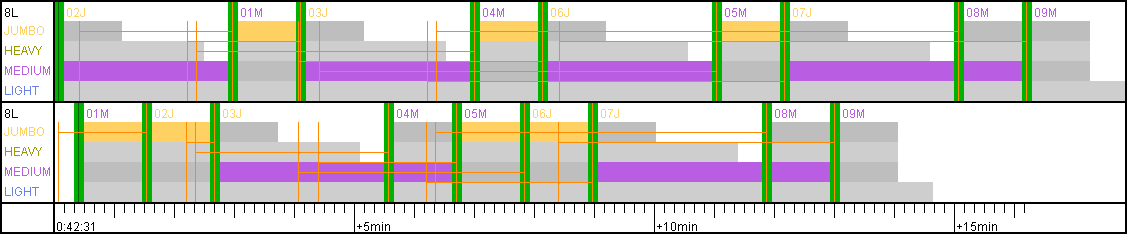
\includegraphics[width=\textwidth]{figures/rwy-eta-order.png}
    \caption{Example of runway plan that preserves the order of estimated time of arrival}
    \label{fig:rwy-eta-order}
\end{figure}

Fourth algorithm schedules the slots in a way that preserves the order of estimated time of arrival. If the slot doesn't fit, any already planned slots following this one are delayed. This way the maximal delay time of each slot is minimized. If there is a continuous string of planes scheduled for approach one after other and new, early arriving plane appears on the radar screen the controller using this algorithm will squeeze the plane in and postpone the planes following in the string. This prevents a situation where the new airplane would wait for all the planes in the string to land first and potentially deplete its fuel supply. On the other hand the controller may need to postpone a significant number of previously planned aircraft which would take a considerable amount of time.

In the example plan shown in Figure \ref{fig:rwy-eta-order} note how the flight \texttt{DAL1043} squeezes before \texttt{DAL508} not affecting any following traffic. In the plan generated by previous algorithm (\ref{fig:rwy-fill-voids}) the flight \texttt{DAL1043} is not even in the visible portion of the plan, delayed by more than \mbox{9 minutes}.

\subsection{Algorithm 5}

Algorithm 5 is an algorithm commonly used in combinatorial optimization and is called Branch and bound. The algorithm is used here in three different variants, each optimizing different criterion. First variant minimizing $C_{max}$, the schedule length also called makespan, which is equal to completion time of last task.  Second variant minimizes $W_{max} = max\{w_j\}$, maximal waiting time. The waiting time is defined as the difference between release time and start time of the task, in this instance difference between required time of arrival and actual time of arrival. Third variant minimizes $\sum{w_j}$, the sum of all waiting times.

\begin{figure}[h]
    \centering
    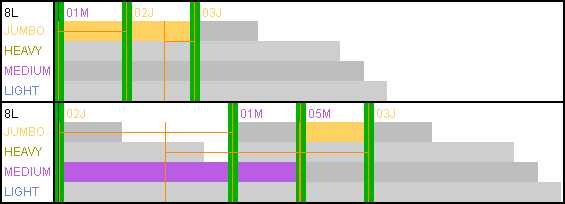
\includegraphics[width=0.7\textwidth]{figures/rwy-proof.png}
    \caption{Example of adding later slot causing changes in plan before its ETA}
    \label{fig:rwy-proof}
\end{figure}

\begin{figure}[h]
    \centering
    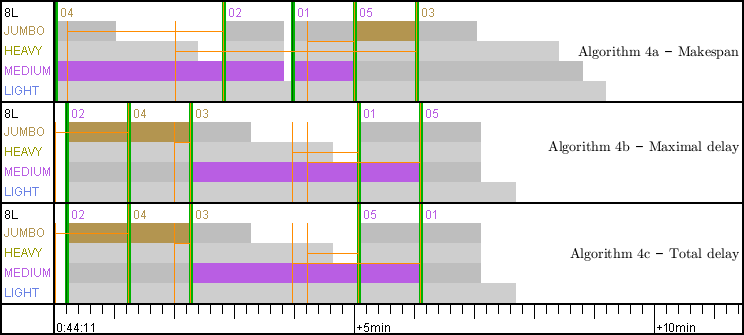
\includegraphics[width=\textwidth]{figures/rwy-bab.png}
    \caption{Comparison between Algorithm 4 (first row) and three variants of Algorithm 5}
    \label{fig:rwy-bab}
\end{figure}
%Můžu boundnout makespan pokud mám seřazené ETA
\red{TODO}

\section{Runway Selection}

\section{STAR Selection}
